%%%%%%%%%%%%%%%%%%%%%%%%%%%%%%%%%%%%%%%%%
% Programming/Coding Assignment
% LaTeX Template
%
% This template has been downloaded from:
% http://www.latextemplates.com
%
% Original author:
% Ted Pavlic (http://www.tedpavlic.com)
%
% Note:
% The \lipsum[#] commands throughout this template generate dummy text
% to fill the template out. These commands should all be removed when 
% writing assignment content.
%
% This template uses a Perl script as an example snippet of code, most other
% languages are also usable. Configure them in the "CODE INCLUSION 
% CONFIGURATION" section.
%
%%%%%%%%%%%%%%%%%%%%%%%%%%%%%%%%%%%%%%%%%

%----------------------------------------------------------------------------------------
%	PACKAGES AND OTHER DOCUMENT CONFIGURATIONS
%----------------------------------------------------------------------------------------

\documentclass{article}

\usepackage{fancyhdr} % Required for custom headers
\usepackage{lastpage} % Required to determine the last page for the footer
\usepackage{extramarks} % Required for headers and footers
\usepackage[usenames,dvipsnames]{color} % Required for custom colors
\usepackage{graphicx} % Required to insert images
\usepackage{subcaption}
\usepackage{listings} % Required for insertion of code
\usepackage{courier} % Required for the courier font
\usepackage{lipsum} % Used for inserting dummy 'Lorem ipsum' text into the template
\usepackage{amsfonts}
\usepackage{amssymb}
\usepackage{amsmath}
\usepackage{enumerate}
\usepackage{soul}
\usepackage[justification=centering]{caption}
%Code for including Python code in Latex - outlined on the Piazza forum post, taken from Stackoverflow

\usepackage{enumitem}
\usepackage[utf8]{inputenc}
\definecolor{dkgreen}{rgb}{0,0.6,0}
\definecolor{gray}{rgb}{0.5,0.5,0.5}
\definecolor{mauve}{rgb}{0.58,0,0.82}

\lstset{frame=tb,
  language=Python,
  aboveskip=3mm,
  belowskip=3mm,
  showstringspaces=false,
  columns=flexible,
  basicstyle={\small\ttfamily},
  numbers=none,
  numberstyle=\tiny\color{gray},
  keywordstyle=\color{blue},
  commentstyle=\color{dkgreen},
  stringstyle=true{mauve},
  breaklines=true,
  breakatwhitespace=true,
  tabsize=3
}

% Margins
\topmargin=-0.45in
\evensidemargin=0in
\oddsidemargin=0in
\textwidth=6.5in
\textheight=9.0in
\headsep=0.25in

% Paragraph spacing
\setlength{\parskip}{10pt}


\linespread{1.1} % Line spacing

% Set up the header and footer
\pagestyle{fancy}
\lhead{\hmwkAuthorName} % Top left header
\chead{\hmwkClass\ (\hmwkClassTime): \hmwkTitle} % Top center head
%\rhead{\firstxmark} % Top right header
\lfoot{\lastxmark} % Bottom left footer
\cfoot{} % Bottom center footer
\rfoot{Page\ \thepage\ of\ \protect\pageref{LastPage}} % Bottom right footer

\setlength\parindent{0pt} % Removes all indentation from paragraphs

%----------------------------------------------------------------------------------------
%	CODE INCLUSION CONFIGURATION
%----------------------------------------------------------------------------------------

\definecolor{MyDarkGreen}{rgb}{0.0,0.4,0.0} % This is the color used for comments
\lstloadlanguages{Perl} % Load Perl syntax for listings, for a list of other languages supported see: ftp://ftp.tex.ac.uk/tex-archive/macros/latex/contrib/listings/listings.pdf
\lstset{language=Perl, % Use Perl in this example
        frame=single, % Single frame around code
        basicstyle=\small\ttfamily, % Use small true type font
        keywordstyle=[1]\color{Blue}\bf, % Perl functions bold and blue
        keywordstyle=[2]\color{Purple}, % Perl function arguments purple
        keywordstyle=[3]\color{Blue}\underbar, % Custom functions underlined and blue
        identifierstyle=, % Nothing special about identifiers                                         
        commentstyle=\usefont{T1}{pcr}{m}{sl}\color{MyDarkGreen}\small, % Comments small dark green courier font
        stringstyle=\color{Purple}, % Strings are purple
        showstringspaces=false, % Don't put marks in string spaces
        tabsize=5, % 5 spaces per tab
        %
        % Put standard Perl functions not included in the default language here
        morekeywords={rand},
        %
        % Put Perl function parameters here
        morekeywords=[2]{on, off, interp},
        %
        % Put user defined functions here
        morekeywords=[3]{test},
       	%
        morecomment=[l][\color{Blue}]{...}, % Line continuation (...) like blue comment
        numbers=left, % Line numbers on left
        firstnumber=1, % Line numbers start with line 1
        numberstyle=\tiny\color{Blue}, % Line numbers are blue and small
        stepnumber=5 % Line numbers go in steps of 5
}

% Creates a new command to include a perl script, the first parameter is the filename of the script (without .pl), the second parameter is the caption
\newcommand{\perlscript}[2]{
\begin{itemize}
\item[]\lstinputlisting[caption=#2,label=#1]{#1.pl}
\end{itemize}
}

%----------------------------------------------------------------------------------------
%	DOCUMENT STRUCTURE COMMANDS
%	Skip this unless you know what you're doing
%----------------------------------------------------------------------------------------

% Header and footer for when a page split occurs within a problem environment
\newcommand{\enterProblemHeader}[1]{
%\nobreak\extramarks{#1}{#1 continued on next page\ldots}\nobreak
%\nobreak\extramarks{#1 (continued)}{#1 continued on next page\ldots}\nobreak
}

% Header and footer for when a page split occurs between problem environments
\newcommand{\exitProblemHeader}[1]{
%\nobreak\extramarks{#1 (continued)}{#1 continued on next page\ldots}\nobreak
%\nobreak\extramarks{#1}{}\nobreak
}

\setcounter{secnumdepth}{0} % Removes default section numbers
\newcounter{homeworkProblemCounter} % Creates a counter to keep track of the number of problems
\setcounter{homeworkProblemCounter}{-1}

\newcommand{\homeworkProblemName}{}
\newenvironment{homeworkProblem}[1][Problem \arabic{homeworkProblemCounter}]{ % Makes a new environment called homeworkProblem which takes 1 argument (custom name) but the default is "Problem #"
\stepcounter{homeworkProblemCounter} % Increase counter for number of problems
\renewcommand{\homeworkProblemName}{#1} % Assign \homeworkProblemName the name of the problem
\section{\homeworkProblemName} % Make a section in the document with the custom problem count
\enterProblemHeader{\homeworkProblemName} % Header and footer within the environment
}{
\exitProblemHeader{\homeworkProblemName} % Header and footer after the environment
}

\newcommand{\problemAnswer}[1]{ % Defines the problem answer command with the content as the only argument
\noindent\framebox[\columnwidth][c]{\begin{minipage}{0.98\columnwidth}#1\end{minipage}} % Makes the box around the problem answer and puts the content inside
}

\newcommand{\homeworkSectionName}{}
\newenvironment{homeworkSection}[1]{ % New environment for sections within homework problems, takes 1 argument - the name of the section
\renewcommand{\homeworkSectionName}{#1} % Assign \homeworkSectionName to the name of the section from the environment argument
\subsection{\homeworkSectionName} % Make a subsection with the custom name of the subsection
\enterProblemHeader{\homeworkProblemName\ [\homeworkSectionName]} % Header and footer within the environment
}{
\enterProblemHeader{\homeworkProblemName} % Header and footer after the environment
}

%----------------------------------------------------------------------------------------
%	NAME AND CLASS SECTION
%----------------------------------------------------------------------------------------

\newcommand{\hmwkTitle}{Assignment 4 \\ Tic-Tae-Toe with Policy Gradient} % Assignment title
\newcommand{\hmwkDueDate}{Friday,\ April 2,\ 2018} % Due date
\newcommand{\hmwkClass}{CSC2515} % Course/class
\newcommand{\hmwkClassTime}{L0101} % Class/lecture time
\newcommand{\hmwkAuthorName}{M.Wong, S.Pyda} % Your name

%----------------------------------------------------------------------------------------
%	TITLE PAGE
%----------------------------------------------------------------------------------------

\title{
\vspace{2in}
\textmd{\textbf{\hmwkClass:\ \hmwkTitle}}\\
\normalsize\vspace{0.1in}\small{Due\ on\ \hmwkDueDate}\\
\vspace{0.1in}
\vspace{3in}
}

\author{\textbf{\hmwkAuthorName}}
%\date{} % Insert date here if you want it to appear below your name

%----------------------------------------------------------------------------------------

\begin{document}

\maketitle
\clearpage
%----------------------------------------------------------------------------------------
%	Introduction
%----------------------------------------------------------------------------------------

\begin{homeworkProblem}

\noindent \textit{Introductory information and readme instructions}

This submissions contains the required files:  \textit{tictactoe.py, tictactoe.tex  \&tictactoe.pdf}. The starter code \textit{tictactoe.py} provided in the project description is used.  Code was written in Python 3.5 with the Anaconda environment. PyTorch 0.31.post2 is used. 


\end{homeworkProblem}
\clearpage
%----------------------------------------------------------------------------------------
%	PROBLEM 1
%----------------------------------------------------------------------------------------

% To have just one problem per page, simply put a \clearpage after each problem

\begin{homeworkProblem}

\noindent \textit{Environment Description}

The starter code \textit{tictactoe.py} provides an \textit{Environment} class, which is a framework for the Tic-Tac-Toe game.  The tictactoe grid is initalized at each new game with \textit{self.grid=np.array([0]*9)}; this is an numpy array of length 9 representing the flattened 3 by 3 grid.  The attribute \textit{turn} represents whose turn it is during the game (e.g. Player 1 vs. Player 2); when the grid is rendered 1 represents 'x' and 2 represents 'o'. After a valid play that does not end the game, the players change from 1 to 2 or vice versa. 
\\

The frozenset \textit{win\_set} contains 8 tuples of length 3. Each tuple contains a winning combination of plays (indices on the grid). If the same label (except for 0) is contained at all three indices, that player wins the game.  This is checked in \textit {check\_win(self)}. The attribute \textit{done} determines if the current game is finished. The game is finished if a player wins or if the grid is full - if the game is finished \textit{self.done=True}.
\\

The \textit{step()} function provides a method for a user/agent to input a move into the gameboard, taking in \textit{action} as it's parameter (e.g. where to place an X/O on the board, represented by a number from 0-9).  The \textit{render()} method shows the current state of the board.  The following code was written to test both functions:
\\  

\begin{lstlisting}
if __name__ == '__main__':
    import sys
    policy = Policy()
    env = Environment()
    if len(sys.argv) == 1:
        # `python tictactoe.py` to train the agent
        train(policy, env)
    else:
        # `python tictactoe.py <ep>` to print the first move distribution
        # using weight checkpoint at episode int(<ep>)
        #ep = int(sys.argv[1])
        #load_weights(policy, ep)
        # print(first_move_distr(policy, env))
        print(env.step(action=4))
        print(env.step(action=1))
        print(env.render())

\end{lstlisting}

The following output was obtained from the execution of the above code.
\begin{lstlisting}
(array([0, 0, 0, 0, 1, 0, 0, 0, 0]), 'valid', False)
(array([0, 2, 0, 0, 1, 0, 0, 0, 0]), 'valid', False)
.o.
.x.
...
\end{lstlisting}

\end{homeworkProblem}
\clearpage
%----------------------------------------------------------------------------------------
%	PROBLEM 2
%----------------------------------------------------------------------------------------

\begin{homeworkProblem}
\noindent \textit{Policy}
\begin{enumerate}[label=(\Alph*)]
\item The implementation for the \textit{TO-DO} sections in the provided Python file is listed below.  The neural network is a fully connected, one hidden layer neural network.
\begin{lstlisting}
class Policy(nn.Module):
    """
    The Tic-Tac-Toe Policy
    """
    def __init__(self, input_size=27, hidden_size=64, output_size=9):
        super(Policy, self).__init__()
        # TODO
        self.features = nn.Sequential(
            nn.Linear(input_size, hidden_size),
            nn.ReLU(inplace=True),
            nn.Linear(hidden_size, output_size)
        )

    def forward(self, x):
        x = self.features(x)
        output = torch.nn.functional.softmax(x, dim=1)
        return output
\end{lstlisting}

\item For a given position on the board, the select\_action function will return the probabilities that the agent should take with respect to the available moves - in this case, either X, O or no action.  As there are 9 total positions on the board, therefore, there are $3x3x3 = 27$ total vector dimensions (e.g. 3 moves per position $\times$ 3 positions per row $\times$ 3 rows per board).

\item Each value in the 9 dimensional output is a probability value representing the best action to take on the board (e.g. $3\times3$ actions) - i.e. the higher the number, the higher the probability of that action being the best action.  The output of the policy is stochastic as it outputs a probability distribution of the best moves based on the current status of the board and not deterministic (e.g. there is no one best move for the current board status).
\end{enumerate}
\end{homeworkProblem}


\clearpage


%----------------------------------------------------------------------------------------
%	PROBLEM 3
%----------------------------------------------------------------------------------------

\begin{homeworkProblem}
\noindent \textit{Policy Gradient}

\begin{enumerate}[label=(\Alph*)]
\item The implementation for the \textit{compute\_returns} function is located below.
\begin{lstlisting}
def compute_returns(rewards, gamma=1.0):
    returns = []
    for index, reward in enumerate(rewards):
        i = index
        exponent = 1
        if i == len(rewards)-1:
            returns.append(reward)
        else:
            while i < len(rewards)-1:
                reward += (gamma**exponent)*(rewards[i+1])
                exponent += 1
                i += 1
            returns.append(reward)
    return returns

\end{lstlisting}

\item The backwards pass to update weights is computed when the entire episode is complete. The weights cannot be updated in the middle of an episode because the final win/lose/tie state (that determines the reward) is not known until the end of the episode. 


\end{enumerate}
\end{homeworkProblem}
\clearpage
%----------------------------------------------------------------------------------------
%	PROBLEM 4
%----------------------------------------------------------------------------------------

\begin{homeworkProblem}
\noindent \textit{Rewards}

\begin{enumerate}[label=(\Alph*)]
\item The \textit{get\_reward} function was modified to the following:
\begin{lstlisting}
def get_reward(status):
    """Returns a numeric given an environment status."""
    return {
            Environment.STATUS_VALID_MOVE  : 0, # TODO
            Environment.STATUS_INVALID_MOVE: -100,
            Environment.STATUS_WIN         : 10,
            Environment.STATUS_TIE         : 0,
            Environment.STATUS_LOSE        : 0
    }[status]

\end{lstlisting}

\item A large penalty (-100) was chosen to signficantly penalize invalid moves to ensure that the agent learned to stop making invalid moves earlier and consider only valid moves.  Per the instructions, and in order for the agent to play the game 'correctly' we chose a penalty (by some trial and error) that ensured the agent played fewer than 3\% invalid moves.  
\\

The only positive reward that was implemented was for winning a match. Each of the other statuses had a zero reward. The intuition here was to not penalize the agent for playing a move that was valid, but also, not penalize the agent for playing moves that resulted in ties or losses, only rewarding the agent for winning moves.
\\

It was observed that by adding rewards for a tie or a negative reward for a loss, the agent was drawn to more ties and fewer wins. This reward system, by trial and error, resulted in very few invalid moves and a win rate of ~90\% by 100,000 episodes. It can be noted that another combination of rewards might achieve similar or better results; the reward system could also depend on what value is placed on each outcome - for example; is the objective to maximize the number of wins, or minimize the number of losses even if there are more ties. 

\end{enumerate}
\end{homeworkProblem}
\clearpage
%----------------------------------------------------------------------------------------
%----------------------------------------------------------------------------------------
%	PROBLEM 5
%----------------------------------------------------------------------------------------

\begin{homeworkProblem}
\noindent \textit{Training}

\begin{enumerate}[label=(\Alph*)]
\item The learning curve for the agent is shown in the following figure.  The number of neurons in the hidden layer was modified to 9 instead of the default 64 from the starter code.
 \begin{center}
\begin{figure}[!ht]\centering
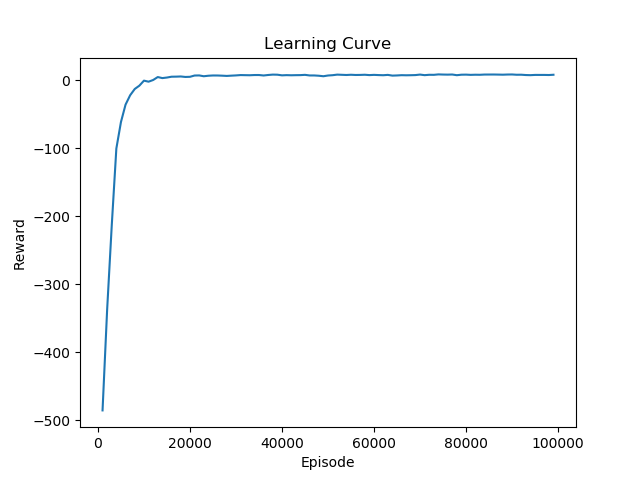
\includegraphics[scale=0.75]{part5.png}
\caption{Learning curve - average return vs. episode number}
\end{figure}
\end{center}
\item  The effect of number of units in the hiddle layer vs. performance of the agent was measured by both increasing and decreasing the number of units and measuring the win rate of the trained agent at 100,000 episodes. The performance was tested with numerous numbers of hidden neurons. The performance with 9, 16, and 64 hidden neurons is shown on the following page.  It can be seen that 9 hidden neurons results in both the best win rate of the trained epsiode at 100,000 episodes and the highest stability (less fluctuation). 

\clearpage

\begin{figure*}[!ht]
\begin{subfigure}{.35\textwidth}\centering
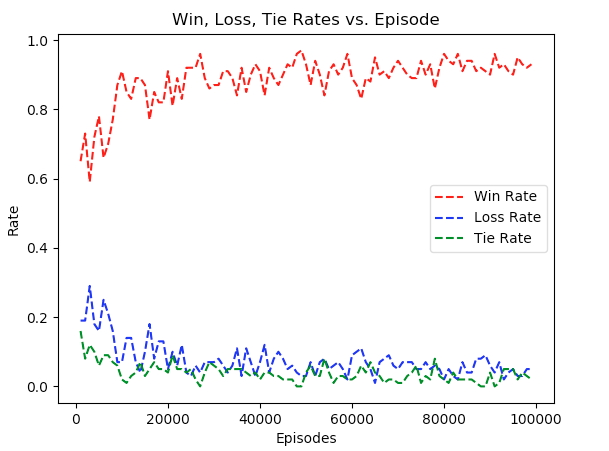
\includegraphics[scale=0.25]{part6a.png}
\caption{9 hidden neurons \\ 100 000 Episodes}
\label{}
\end{subfigure}
\begin{subfigure}{.35\textwidth}\centering
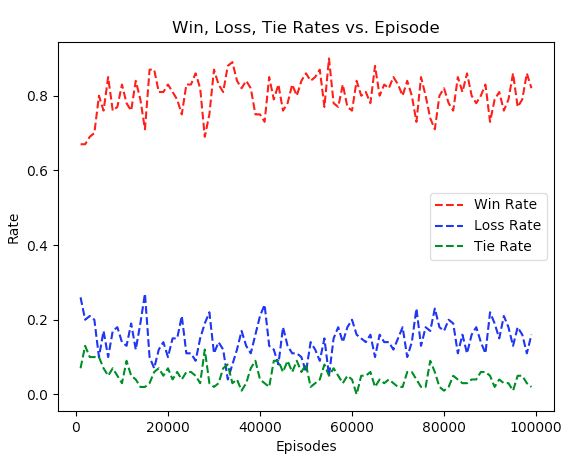
\includegraphics[scale=0.25]{part6c.png}
\caption{18 hidden neurons \\100 000 Episodes}
\label{}
\end{subfigure}%
\begin{subfigure}{.35\textwidth}\centering
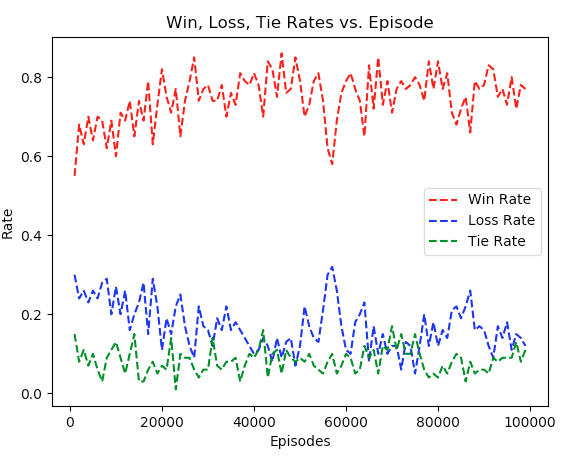
\includegraphics[scale=0.25]{part6e.png}
\caption{64 hidden neurons \\ 100 000 Episodes}
\label{}
\end{subfigure}
\begin{subfigure}{.35\textwidth}\centering
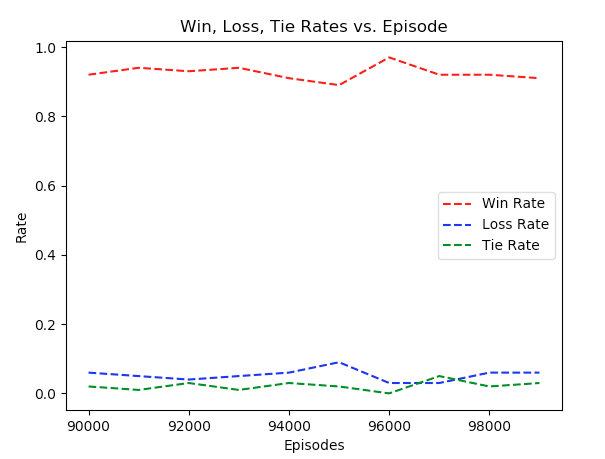
\includegraphics[scale=0.25]{part6b.png}
\caption{9 hidden neurons\\ Final 10 000 Episodes}
\label{}
\end{subfigure}%
\begin{subfigure}{.35\textwidth}\centering
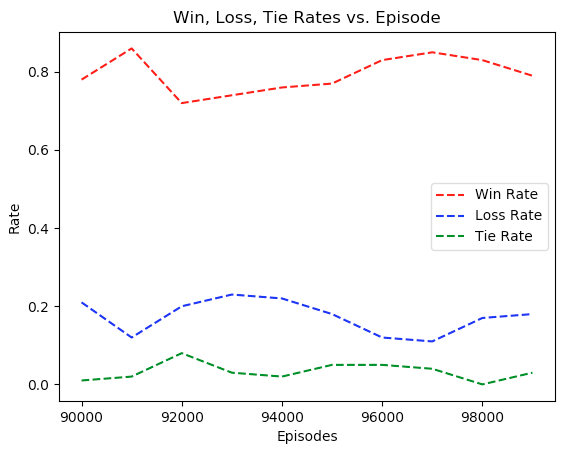
\includegraphics[scale=0.25]{part6d.png}
\caption{18 hidden neurons \\ Final 10 000 Episodes}
\label{}
\end{subfigure}
\begin{subfigure}{.35\textwidth}\centering
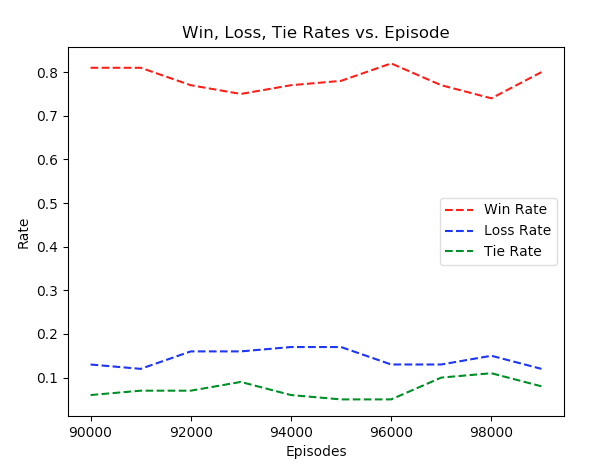
\includegraphics[scale=0.25]{part6f.png}
\caption{64 hidden neurons \\ Final 10 000 Episodes}
\label{}%
\end{subfigure}
\caption{Tic-Tac-Toe agent performance with number of hidden neurons (all episodes on top and last 10000 below}
\label{fig:pcs}
\end{figure*}

\item  Based on the choice of rewards and number of units in the hidden layer, we observed that agent stopped playing invalid moves at approximately episode 25000.  To obtain this answer, we fetched the environment status every time an agent played an invalid move and incremented the total number of invalid moves by 1.  The total numnber of invalid moves was then output to the console. Some examples of the output are shown below. 

\begin{lstlisting}

python tictactoe.py 30000
Number of games won: 90
Number of games tied: 1
Number of games lost: 9
Number of invalid moves: 1

python tictactoe.py 50000
Number of games won: 88
Number of games tied: 1
Number of games lost: 11
Number of invalid moves: 0

python tictactoe.py 99000
Number of games won: 90
Number of games tied: 1
Number of games lost: 9
Number of invalid moves: 0

\end{lstlisting}

\item After running the agent for 100000 episodes, we were able to obtain a win rate of approximately 88-90\% (the reason for a range was due to the fact that an issue with seeding any random functionality was not resolved in time for this report).  The loss rate fluctuated between 15-20\% and the tie rate was the remaining percentage of games played.  The following output displays the first 5 games played by our agent, given a set of policy weights:
\begin{lstlisting}
# Game 1
xo.
ox.
..x
====
# Game 2
x..
.x.
oox
====
# Game 3
xo.
.x.
o.x
====
# Game 4
x.x
oxo
o.x
====
# Game 5
xo.
.xo
..x
====

\end{lstlisting}
\end{enumerate}


\end{homeworkProblem}
\clearpage
%----------------------------------------------------------------------------------------
%----------------------------------------------------------------------------------------
%	PROBLEM 6
%----------------------------------------------------------------------------------------

\begin{homeworkProblem}
\noindent \textit{Win Rate over Episodes}

The following graphs outlines the win, lose, and tie rates for the agent vs. episode for 9 hidden neurons (the chosen hyperparameter). 

\begin{figure}[!ht]\centering
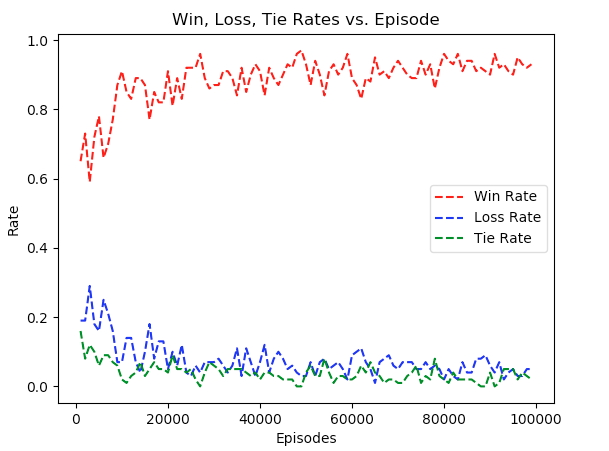
\includegraphics[scale=0.4]{part6a.png}
\caption{Win/Lose/Tie rates vs. episode - 100 000 Episodes}
\end{figure}

\begin{figure}[!ht]\centering
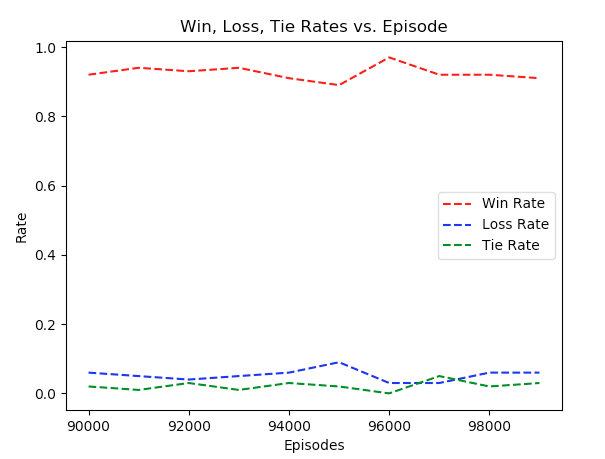
\includegraphics[scale=0.4]{part6b.png}
\caption{Win/Lose/Tie rates vs. episode - Final 10 000 Episodes}
\end{figure}

Given that a random agent playing the game results in a win rate of approximately 60\%, it appears that the agent is learning effectively enough to net a win rate that is higher than if a random agent was playing the game.  The three lines in the figure however, are quite noisy (e.g. they do not follow a smooth pattern), perhaps indicating that the hyperparameters could be tuned some more.


\end{homeworkProblem}
\clearpage
%----------------------------------------------------------------------------------------
%	PROBLEM 7
%----------------------------------------------------------------------------------------
\begin{homeworkProblem}
\noindent \textit{First Move Distribution Over Episodes}

The first move distribution earlier in the training process at 5000 episodes was as follows:
\begin{lstlisting}
 0.1057  0.0288  0.1239  0.0201  0.1903  0.0298  0.0295  0.0178  0.4542
[torch.FloatTensor of size 1x9]
\end{lstlisting}

Similarly, at 50000 episodes:
\begin{lstlisting}
Columns 0 to 5 
 2.1984e-03  3.3832e-06  2.3268e-02  1.0383e-05  2.6650e-02  3.1879e-05

Columns 6 to 8 
 1.6433e-03  2.6558e-05  9.4617e-01
[torch.FloatTensor of size 1x9]
\end{lstlisting}

For the final trained model:
\begin{lstlisting}
Columns 0 to 5 
 2.6256e-03  2.1233e-07  1.4166e-03  7.9190e-07  2.9096e-03  2.9352e-06

Columns 6 to 8 
 2.4797e-03  2.8529e-06  9.9056e-01
[torch.FloatTensor of size 1x9]

\end{lstlisting}

The output of the last function call indicates that the agent has learned that playing in the corner position is the best possible move, as evidenced from the 0.99056 value in Column 8.  Earlier in the training process, we observe that the policy is learning which position to play first and already at 5000 episodes, the bottom right hand corner is already selected as the optimal first move.


\end{homeworkProblem}
\clearpage
%----------------------------------------------------------------------------------------
%	PROBLEM 8
%----------------------------------------------------------------------------------------
\begin{homeworkProblem}
\noindent \textit{Limitations}

As discussed in Part 7, the trained agent is most likely to play first in the bottom right corner of the board.  The main limitation of the trained agent is that while it correctly learned the optimal first position in the game, it loses against a random policy.  Theoretically, the worst outcome for an optimal first move in this game (e.g. one of the corner positions) is a tie.  The agent appear to play moves that would result in a loss, such as in the following example:
\begin{lstlisting}
x.x
ooo
xox
\end{lstlisting}

This example illustrates that the first move carried out by the agent was in the bottom right corner, yet still lost against a random player.


\end{homeworkProblem}
\clearpage

\end{document}



